\section{Intermezzo}
\label{sec:intermezzo}

\begin{frame}
	\frametitle{Intermezzo: Matrix multiplication}
	\begin{columns}
		\column{0.455\textwidth}
		\begin{problemblock}{Matrix multiplication}
			Compute $A \times B$, where $A$ and $B$ are $n$-by-$n$ matrices.	
		\end{problemblock}
		\begin{answerblock}{How do we do that?}
			\begin{itemize}
				\item Remember that $c_{i,j} = \sum\limits_{k=1}^n a_{i,k}b_{k,j}$.
				\item So for every cell $c_{i,j}$, we need $O(n)$ multipliations and additions.
				\item There are $n^2$ cells, so $O(n^3)$ work in total.
			\end{itemize}
		\end{answerblock}
		\column{0.455\textwidth}
	\begin{center}
		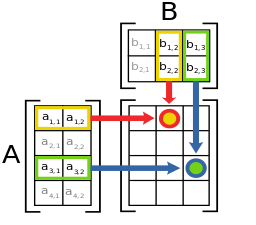
\includegraphics[width=0.8\textwidth]{figures/matrix_multiplication.png}\\
		\hspace*{15pt}\hbox{\scriptsize Image By:\thinspace{\itshape Wikimedia user Bilou}}
		% https://commons.wikimedia.org/wiki/File:Matrix_multiplication_diagram_2.svg
	\end{center}
	\end{columns}
\end{frame}
	
\begin{frame}
	\frametitle{Can we do better?}
	
	\begin{itemize}
		\item We can do better! By using \textit{recursion} we need only multiply 7 matrices of size $n/2$ and this gives us
			$O(n^{2.81})$ work!
			\pause
		\item But Pan shows in 1980 that we can multiply two $70$-by-$70$ matrices using \alert{only} 143,640 scalar
			multiplications.
		\item This is $O(n^{2.795})$.
			\pause
		\item This obviously beats the $O(n^{2.81})$ that we had before!
	\end{itemize}
\end{frame}

\begin{frame}
	\frametitle{And so it begins}
	\begin{center}
		
\includegraphics[width=0.8\textwidth]{figures/soitbegins.jpg}
		\hspace*{15pt}\hbox{\scriptsize Image from: \thinspace{\itshape The Lord of the Rings: The Two Towers}}
	\end{center}
\end{frame}

\begin{frame}
	\frametitle{The decimal wars}
	\begin{itemize}
		\item 1969: The one that started it (Strassen) with $O(n^{2.81})$.
			\pause
		\item December 1979: $O(n^{2.521813})$
			\pause
		\item January 1980: \pause $O(n^{2.521801})$
			\pause
		\item 1987: \pause $O(n^{2.376})$
			\pause
		\item 25 years later.... 2012: \pause $O(n^{2.3727})$
			\pause
		\item In fact people now believe a method of $O(n^{2+\epsilon})$ for any $\epsilon > 0$ may exist.
			\pause
		\item But implementation-wise any improvement over Strassen from 1969 (with $O(n^{2.81})$) is less practical.
	\end{itemize}
\end{frame}


